%%%%%%%%%%%%%%%%%%%%% {{{
%%Options for presentations (in-class) and handouts (e.g. print).
\documentclass[pdf,9pt]{beamer}
% \documentclass[pdf,9pt]{beamer}


%%%%%%%%%%%%%%%%%%%%%%
%Change this for different slides so it appears in bar
\usepackage{authoraftertitle}
\date{Chapter 5. Vector Space $\R^n$ \\ \S 5-2. Independence and Dimension}

%%%%%%%%%%%%%%%%%%%%%%
%% Upload common style file
\usepackage{LyryxLAWASlidesStyle}

\begin{document}

%%%%%%%%%%%%%%%%%%%%%%%
%% Title Page and Copyright Common to All Slides

%Title Page
\input frontmatter/titlepage.tex

%LOTS Page
\input frontmatter/lyryxopentexts.tex

%Copyright Page
\input frontmatter/copyright.tex

%%%%%%%%%%%%%%%%%%%%%%%%% }}}
%-------------- start slide -------------------------------%{{{ 2
\begin{frame}[fragile]
   \tableofcontents
\end{frame}
%-------------- end slide -------------------------------%}}}
\section[\textcolor{yellow}{}]{\textcolor{yellow}{Linear Independence}}
%-------------- start slide -------------------------------%{{{ 3
\frame{
\frametitle{Linear Independence}
\pause
\begin{definition}
    Let $S=\{\vec{x}_1, \vec{x}_2, \ldots, \vec{x}_k\}$ be a subset
    of $\RR^n$.  The set $S$ is \alert{linearly independent} (or simply
    independent) if the following condition is satisfied:
    \medskip

    \alert{
	\[t_1\vec{x}_1 + t_2\vec{x}_2 + \cdots + t_k\vec{x}_k=\vec{0}_n	\quad\Rightarrow\quad t_1=t_2=\cdots=t_k=0
    \]}
    \medskip

    i.e., the only linear combination of vectors of $S$ that vanishes
    (is equal to the zero vector) is the trivial one
    (all coefficients equal to zero).

    A set that is {\bf not} linearly independent is called \textcolor{lgtblue}{dependent}.
\end{definition}
}
%-------------- end slide -------------------------------%}}}
%-------------- start slide -------------------------------%{{{ 4
\begin{frame}
   \begin{center}
       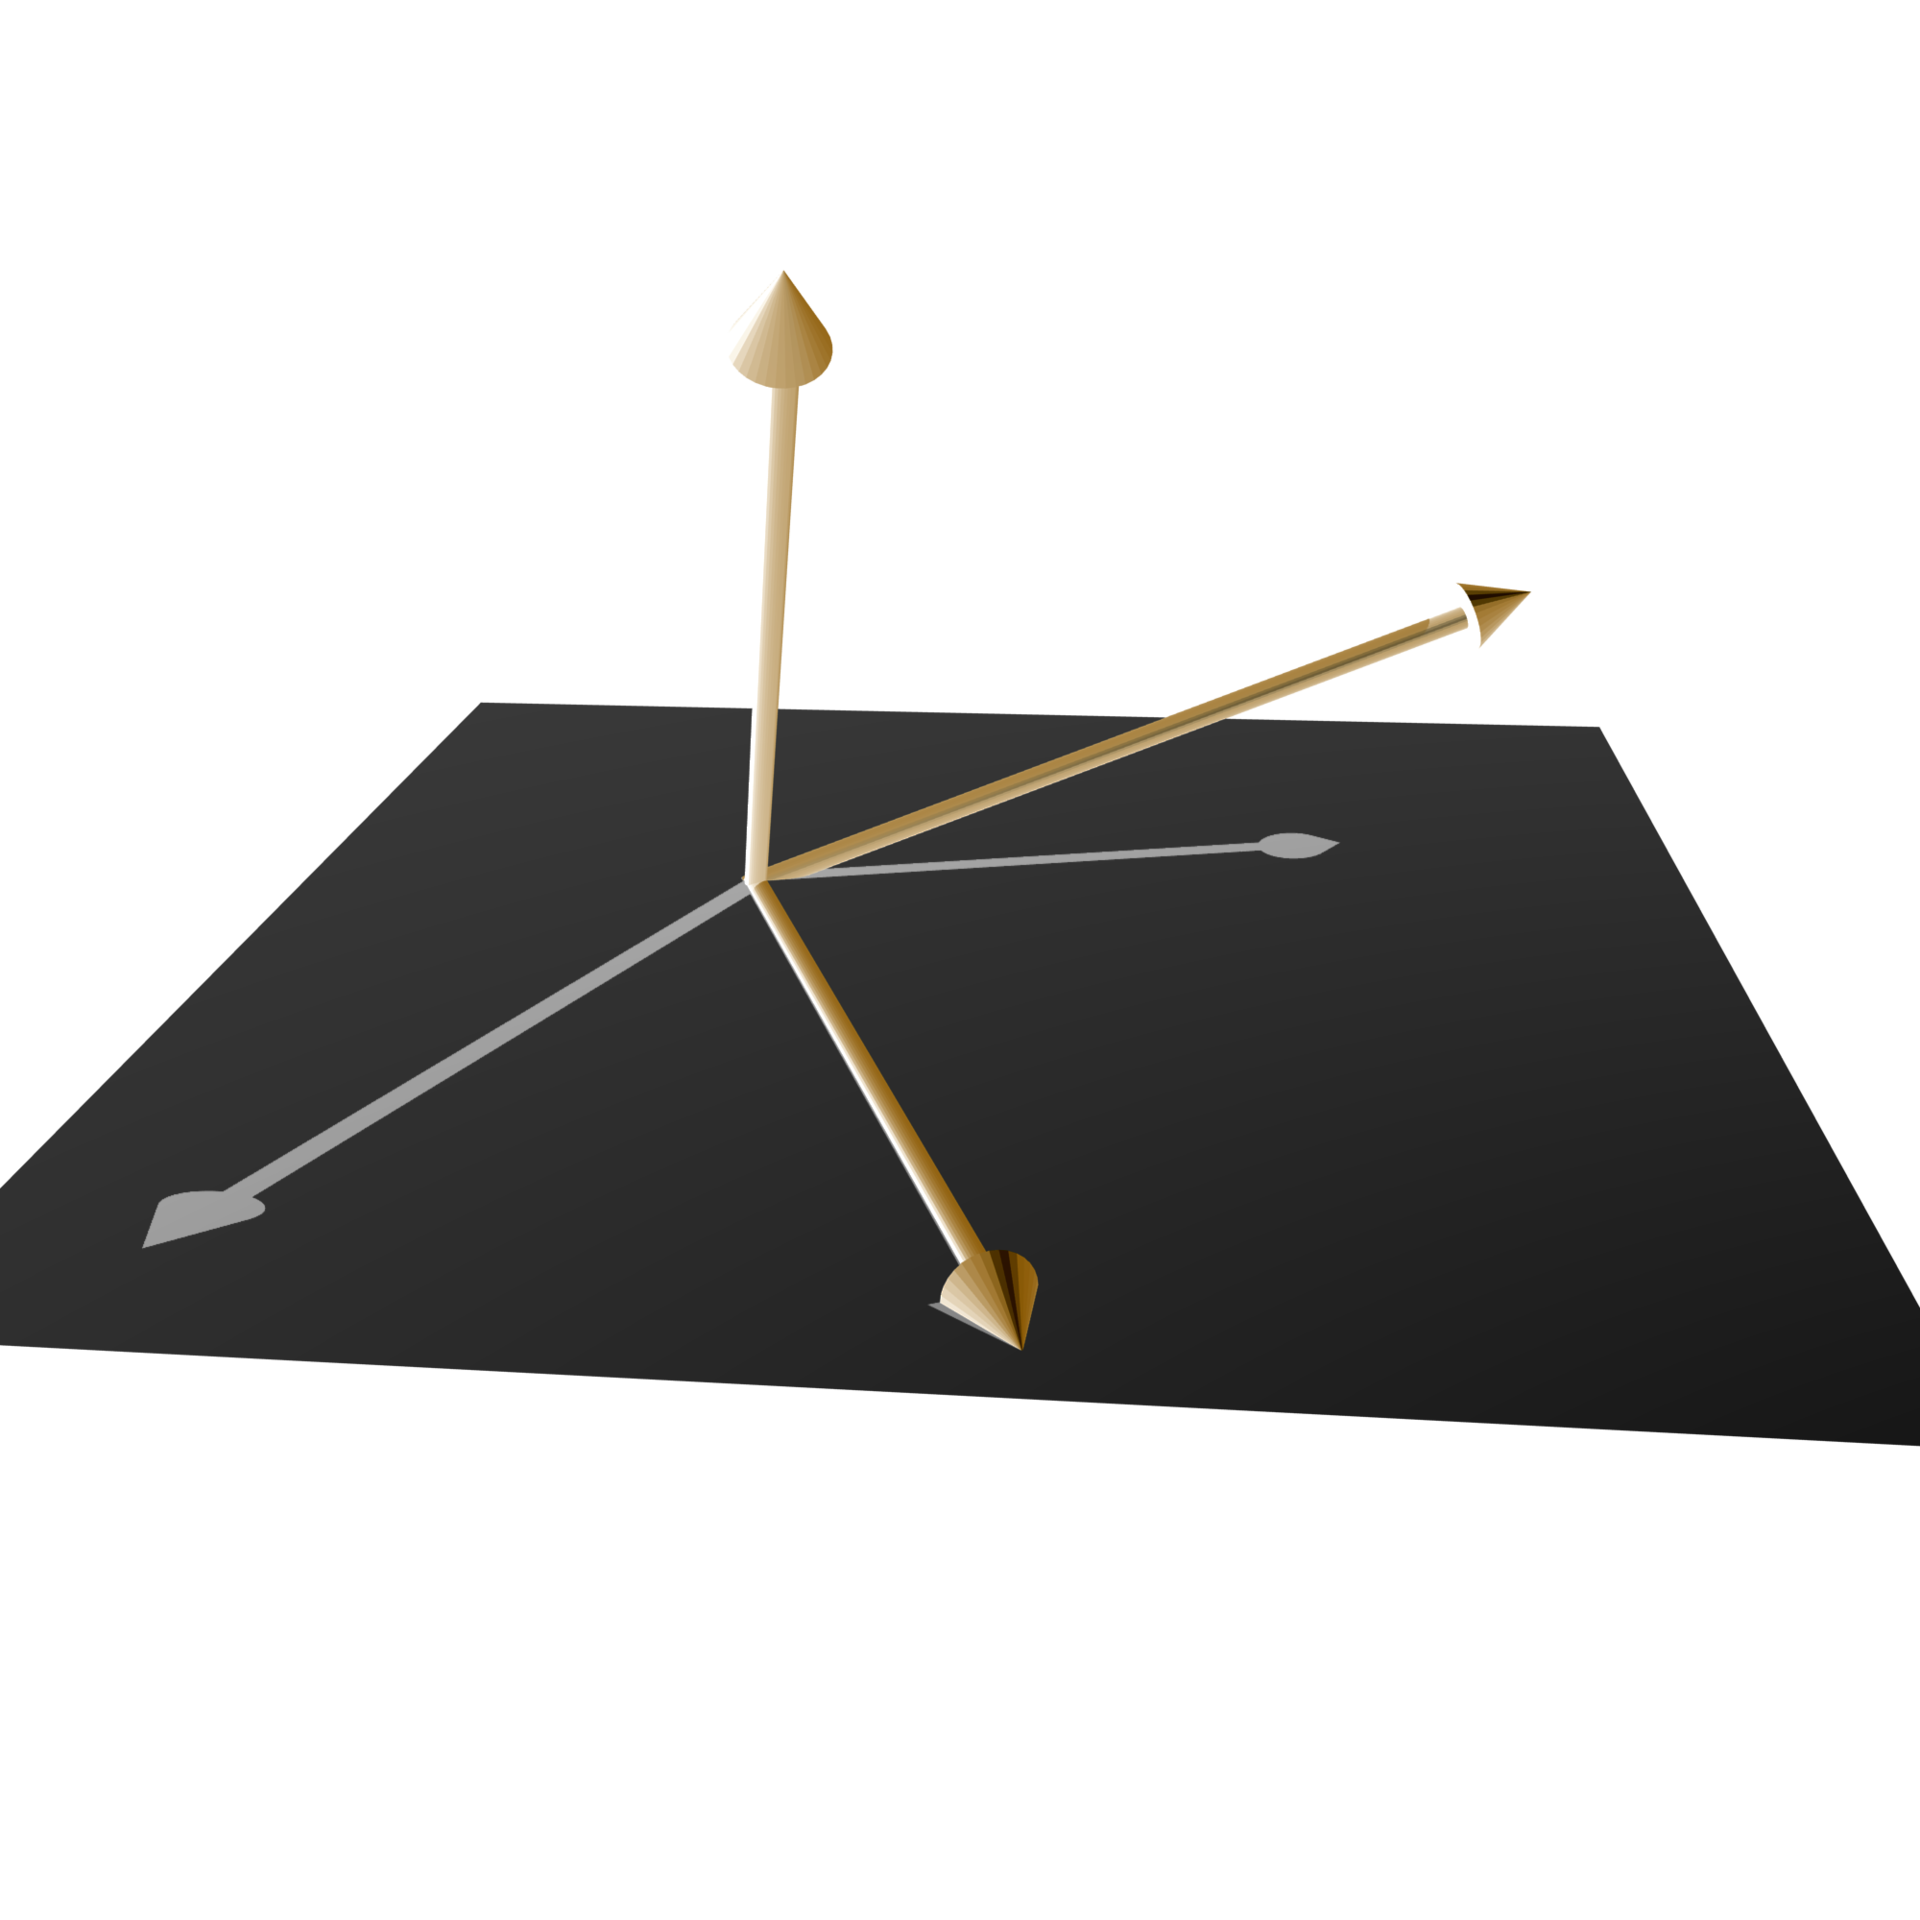
\includegraphics[scale=0.07]{./figures/Vec-indep-neg.png}
   \end{center}
\end{frame}
%-------------- end slide -------------------------------%}}}
%-------------- start slide -------------------------------%{{{ 5
\begin{frame}
   \begin{center}
       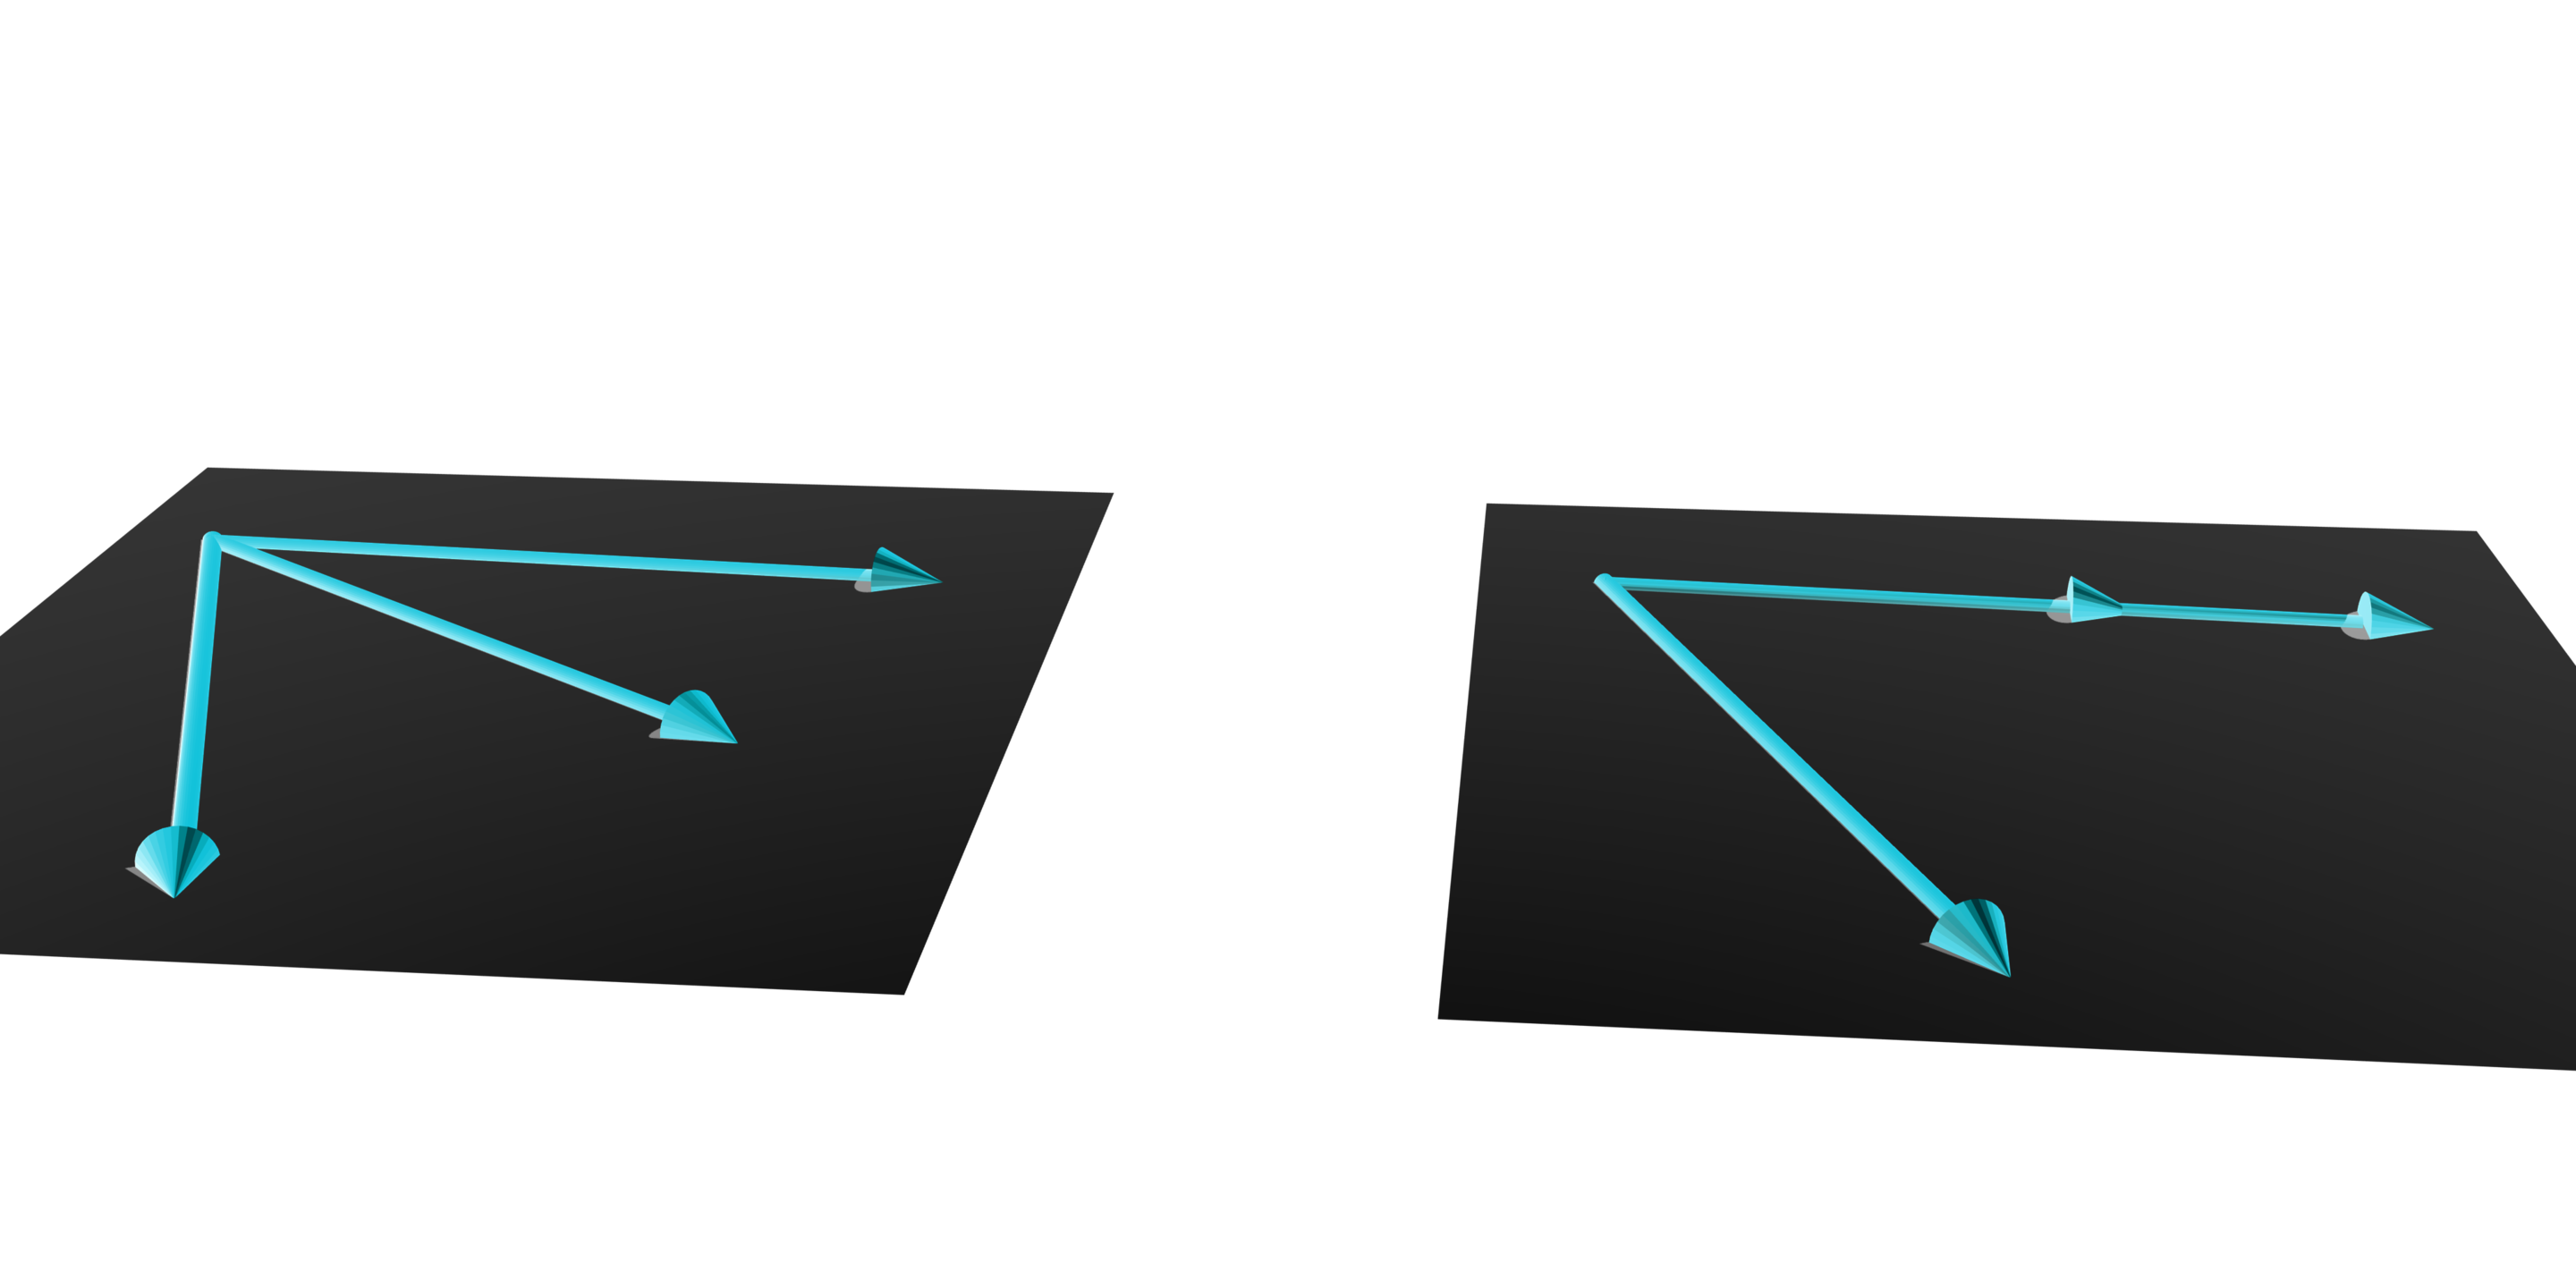
\includegraphics[scale=0.07]{./figures/Vec-dep-neg.png}
   \end{center}
\end{frame}
%-------------- end slide -------------------------------%}}}
%-------------- start slide -------------------------------%{{{ 6
\begin{frame}
    \begin{align*}
    \begin{array}{ ccc }
	\left\{\vec{x}_1,\vec{x}_2,\cdots,\vec{x}_k \right\} &                     & t_1\vec{x}_1 + t_2\vec{x}_2 + \cdots + t_k\vec{x}_k=\vec{0}_n \\ [1em] \hline \\ [1em]
	\textcolor{yellow}{\text{Linearly Independent}}      & \Longleftrightarrow & \textcolor{yellow}{\text{Trivial Solution}}                   \\ [2em]
	\textcolor{lgtblue}{\text{Linearly Dependent}}       & \Longleftrightarrow & \textcolor{lgtblue}{\text{Nontrivial Solution}}
	\end{array}
    \end{align*}
\end{frame}
%-------------- end slide -------------------------------%}}}
%-------------- start slide -------------------------------%{{{ 7
\begin{frame}
\begin{example}
    Is $S=\left\{
	\left[\begin{array}{r} -1 \\ 0 \\ 1 \end{array}\right],
	\left[\begin{array}{r} 1  \\ 1 \\ 1 \end{array}\right],
	\left[\begin{array}{r} 1  \\ 3 \\ 5 \end{array}\right]
    \right\}$
    linearly independent?
    \medskip
    \pause

    Suppose that a linear combination of these vectors vanishes, i.e.,
    there exist $a,b,c\in\RR$ so that
    % \vspace*{-.15in}

    \[
	a\left[\begin{array}{r}  -1 \\ 0 \\ 1 \end{array}\right]
	+b\left[\begin{array}{r} 1  \\ 1 \\ 1 \end{array}\right]
	+c\left[\begin{array}{r} 1  \\ 3 \\ 5 \end{array}\right]
	=\left[\begin{array}{r}  0  \\ 0 \\ 0 \end{array}\right].
    \]
\end{example}

\end{frame}
%-------------- end slide -------------------------------%}}}
%-------------- start slide -------------------------------%{{{ 8
\frame{

\begin{example}[continued]
    Solve the homogeneous system of three equation in three variables:
    \pause
    \[ \left[\begin{array}{rrr|r}
	-1 & 1 & 1 & 0 \\
	0  & 1 & 3 & 0 \\
	1  & 1 & 5 & 0
    \end{array}\right]
    \rightarrow \cdots \rightarrow
    \left[\begin{array}{rrr|r}
	1 & 0 & 2 & 0 \\
	0 & 1 & 3 & 0 \\
	0 & 0 & 0 & 0
    \end{array}\right] .
    \]
    The system has solutions $a=-2r, b=-3r, c=r$ for $r\in\RR$,
    so it has \textcolor{lgtblue}{nontrivial} solutions.
    Therefore $S$ is \textcolor{lgtblue}{dependent}.
    \pause
    In particular, when $r=1$ we see that
    \[
	-2\left[\begin{array}{r} -1 \\ 0 \\ 1 \end{array}\right]
	-3\left[\begin{array}{r} 1  \\ 1 \\ 1 \end{array}\right]
	+\left[\begin{array}{r}  1  \\ 3 \\ 5 \end{array}\right]
	=\left[\begin{array}{r}  0  \\ 0 \\ 0 \end{array}\right],
    \]
    i.e., this is a nontrivial linear combination that vanishes.
\end{example}
}
%-------------- end slide -------------------------------%}}}
%-------------- start slide -------------------------------%{{{ 9
\frame{

\begin{example}
    Consider the set
    $\{ \vec{e}_1, \vec{e}_2, \ldots, \vec{e}_n\}\subseteq \RR^n$,
    and suppose $t_1, t_2, \ldots, t_n\in\RR$ are such that
    \[ t_1\vec{e}_1 + t_2\vec{e}_2 + \cdots t_n\vec{e}_n =\vec{0}_n.\]
    Since
    \[ t_1\vec{e}_1 + t_2\vec{e}_2 + \cdots t_n\vec{e}_n =
    \left[\begin{array}{r} t_1 \\ t_2 \\ \vdots \\ t_n \end{array}\right],
    \]
    the only linear combination that vanishes is the trivial one,
    i.e., the one with $t_1=t_2=\cdots=t_n=0$.
    Therefore, $\{ \vec{e}_1, \vec{e}_2, \ldots, \vec{e}_n\}$
    is linearly independent.
\end{example}
}
%-------------- end slide -------------------------------%}}}
%-------------- start slide -------------------------------%{{{ 10
\frame{
\begin{problem}
    Let $\{\vec{u},\vec{v},\vec{w}\}$ be an independent subset of $\RR^n$.
    Is $\{\vec{u+v}, 2\vec{u+w}, \vec{v}-5\vec{w}\}$ linearly
    independent?
\end{problem}

\pause
\begin{solution}
    In order to show the $\{\vec{u+v}, 2\vec{u+w}, \vec{v}-5\vec{w}\}$ is
    linearly independent, we need to show that
    \begin{align*}
        a(\vec{u}+\vec{v}) + b(2\vec{u}+\vec{w}) + c(\vec{v}-5\vec{w})=\vec{0}_n
	\quad\Rightarrow \quad
	a= b=c=0.
    \end{align*}
    \vspace{-1em}
    \pause
    \[\Updownarrow\]
    \[ (a+2b)\vec{u} + (a+c)\vec{v} + (b-5c)\vec{w}=\vec{0}_n.\]
    \pause
    because $\{\vec{u},\vec{v},\vec{w}\}$ is \textcolor{yellow}{independent} \qquad
    $\Downarrow$
    \begin{eqnarray*}
	a + 2b & = & 0 \\
	a + c  & = & 0 \\
	b - 5c & = & 0 .
    \end{eqnarray*}
    \vspace{-1em}
    \pause
    \[\Downarrow\]
    \[a=b=c=0\]
    % This system of three equations in three variables has
    % the unique solution $a=b=c=0$.
    % Therefore, $\{\vec{u}+\vec{v}, 2\vec{u}+\vec{w}, \vec{v}-5\vec{w}\}$
    % is independent.
    \myQED
\end{solution}
}
%-------------- end slide -------------------------------%}}}
%-------------- start slide -------------------------------%{{{ 11
\frame{
\begin{problem}
    Let $X\subseteq \RR^n$ and suppose that $\vec{0}_n\in X$.
    Show that $X$ linearly dependent.
\end{problem}
\pause
\vfill
\begin{solution}
    Let $X=\{ \vec{x_1}, \vec{x_2}, \ldots, \vec{x_k}\}$ for some
    $k\geq 1$, and suppose $\vec{x}_1=\vec{0_n}$.
    Then
    \[ 1 \vec{x}_1 + 0\vec{x}_2 + \cdots + 0\vec{x}_k =
    1 \vec{0}+ 0\vec{x}_2 + \cdots + 0\vec{x}_k = \vec{0},\]
    i.e., we have found a nontrivial linear combination of the
    vectors of $X$ that vanishes.
    Therefore, $X$ is \textcolor{lgtblue}{dependent}.
    \myQED
\end{solution}
}
%-------------- end slide -------------------------------%}}}
%-------------- start slide -------------------------------%{{{ 12
\frame{
\begin{example}
    Let $\vec{u}\in\RR^n$ and let $S=\{\vec{u}\}$.
    \begin{enumerate}
	\item If $\vec{u}=\vec{0}_n$, then $S$ is \textcolor{lgtblue}{dependent} (see the previous Problem).
	\item If $\vec{u}\neq\vec{0}_n$, then $S$ is \textcolor{yellow}{independent}: if $t\vec{u}=\vec{0}_n$ for some $t\in\RR$, then $t=0$.
    \end{enumerate}
    As a consequence,\\[1em]
    \begin{align*}
	\text{$S=\{\vec{u}\}$ is \textcolor{yellow}{independent}}
     \qquad\Longleftrightarrow\qquad
     \vec{u}\neq\vec{0}_n
    \end{align*}
\end{example}
}
%-------------- end slide -------------------------------%}}}
%-------------- start slide -------------------------------%{{{ 13
\frame{
\begin{example}
    $A=\left[
    \begin{array}{rrrrrr}
	0 & 1 & -1 & 2  & 5 & 1  \\
	0 & 0 & 1  & -3 & 0 & 1  \\
	0 & 0 & 0  & 0  & 1 & -2 \\
	0 & 0 & 0  & 0  & 0 & 0
    \end{array}\right]$ is a row-echelon matrix.
    \pause
    Treat the \alert{nonzero} rows of $A$ as transposes of vectors
    in $\RR^6$:
    \[
	\vec{u}_1= \left[\begin{array}{r} 0 \\ 1 \\ -1 \\ 2  \\ 5 \\ 1  \end{array}\right],\quad
	\vec{u}_2= \left[\begin{array}{r} 0 \\ 0 \\ 1  \\ -3 \\ 0 \\ 1  \end{array}\right],\quad
	\vec{u}_3= \left[\begin{array}{r} 0 \\ 0 \\ 0  \\ 0  \\ 1 \\ -2 \end{array}\right],
    \]
    and suppose that $a\vec{u}_1 +b\vec{u}_2 + c\vec{u}_3=\vec{0}_6$ for some
    $a,b,c\in\RR$.
\end{example}
}
%-------------- end slide -------------------------------%}}}
%-------------- start slide -------------------------------%{{{ 14
\frame{
    \begin{example}[continued]
	This results in a system of six equations in three variables, whose
	augmented matrix is
	\[
	    \left[ \begin{array}{rrr|r}
		    0  & 0  & 0  & 0 \\
		    1  & 0  & 0  & 0 \\
		    -1 & 1  & 0  & 0 \\
		    2  & -3 & 0  & 0 \\
		    5  & 0  & 1  & 0 \\
		    1  & 1  & -2 & 0
	    \end{array}\right] \]
	    \pause
	    The solution to the system is easily determined to be
	    $a=b=c=0$, so the set $\{ \vec{u}_1, \vec{u_2}, \vec{u}_3\}$
	    is \textcolor{yellow}{independent}.
	    \pause Hence,
	    \textcolor{yellow}{nonzero rows of $A$ are independent.}
	\end{example}
	\pause
	\vfill
	\begin{remark}
	    In general, the nonzero rows of any row-echelon matrix form an independent set of (row) vectors.
	\end{remark}
}
%-------------- end slide -------------------------------%}}}
%-------------- start slide -------------------------------%{{{ 15
\frame{
\begin{theorem}
    Let $U=\{ \vec{v}_1, \vec{v}_2, \ldots, \vec{v}_k\} \subseteq\RR^n$
    be an \textcolor{yellow}{independent} set.
    Then any vector $\vec{x}\in\Span(U)$ has a \alert{unique}
    representation as a linear combination of vectors of $U$.
\end{theorem}
\pause
\begin{proofnoend}
    Suppose that there is a vector $\vec{x}\in \Span(U)$ such that
    \begin{eqnarray*}
	\vec{x} & = & s_1\vec{v}_1 + s_2\vec{v}_2 + \cdots + s_k\vec{v}_k, \mbox{ for some } s_1, s_2, \ldots, s_k\in\RR, \mbox{ and} \\
	\vec{x} & = & t_1\vec{v}_1 + t_2\vec{v}_2 + \cdots + t_k\vec{v}_k, \mbox{ for some } t_1, t_2, \ldots, t_k\in\RR.
    \end{eqnarray*}
    \pause
    \vspace{-1em}
    \[\Downarrow\]
    \vspace{-2em}
    \begin{eqnarray*}
	\vec{0}_n  =  \vec{x}-\vec{x}
                  & = & (s_1\vec{v}_1 + s_2\vec{v}_2 + \cdots + s_k\vec{v}_k) -(t_1\vec{v}_1 + t_2\vec{v}_2 + \cdots + t_k\vec{v}_k) \\
                  & = & (s_1-t_1)\vec{v}_1 + (s_2-t_2)\vec{v}_2 + \cdots + (s_k-t_k)\vec{v}_k.
    \end{eqnarray*}
    \pause
    \vspace{-1em}
    \[\hspace{-2em}\text{\textcolor{yellow}{$U$ is independent}}\quad \Downarrow\]
    \begin{align*}
	s_1-t_1=0,\quad s_2-t_2=0,\quad\cdots,s_k-t_k=0
    \end{align*}
    \pause
    \vspace{-2em}
    \[\Updownarrow\]
    \vspace{-2em}
    \begin{align*}
	s_1=t_1,\quad s_2=t_2,\quad\cdots,s_k=t_k.
    \end{align*}
    \myQED
\end{proofnoend}
}
%-------------- end slide -------------------------------%}}}
\section[\textcolor{yellow}{}]{\textcolor{yellow}{Geometric Examples}}
%-------------- start slide -------------------------------%{{{ 16
\frame{
\frametitle{Two Geometric Examples}
\pause
\begin{problem}
    Suppose that $\vec{u}$ and $\vec{v}$ are nonzero vectors in $\RR^3$.
    Prove that $\{ \vec{u},\vec{v}\}$ is \textcolor{lgtblue}{dependent} if and only if
    $\vec{u}$ and $\vec{v}$ are parallel.
\end{problem}
\pause
\vfill
\begin{solution}
    ($\Rightarrow$) If $\{ \vec{u},\vec{v}\}$ is
    \textcolor{lgtblue}{dependent}, then there exist $a,b\in\RR$ so that
    $a\vec{u}+b\vec{v}=\vec{0}_3$ \alert{with $a$ and $b$ not both zero}.  By
    symmetry, we may assume that $a\neq 0$.  Then
    $\vec{u}=-\frac{b}{a}\vec{v}$, so $\vec{u}$ and $\vec{v}$ are scalar
    multiples of each other, i.e., $\vec{u}$ and $\vec{v}$ are parallel.
    \pause
    \bigskip

    ($\Leftarrow$)
    Conversely, if $\vec{u}$ and $\vec{v}$ are parallel, then there
    exists a $t\in\RR$, \alert{$t\neq 0$}, so that $\vec{u}=t\vec{v}$.
    Thus $\vec{u}-t\vec{v}=\vec{0}_3$, so we have a nontrivial linear
    combination of $\vec{u}$ and $\vec{v}$ that vanishes.  Therefore, $\{
    \vec{u},\vec{v}\}$ is \textcolor{lgtblue}{dependent}.\myQED
\end{solution}
}
%-------------- end slide -------------------------------%}}}
%-------------- start slide -------------------------------%{{{ 17
\frame{
\begin{problem}
  Suppose that $\vec{u},\vec{v}$ and $\vec{w}$ are nonzero vectors in $\RR^3$,
  and that $\{ \vec{v},\vec{w}\}$ is independent.  Prove that $\{
  \vec{u},\vec{v},\vec{w}\}$ is \textcolor{yellow}{independent} if and only if
  $\vec{u}\not\in\Span\{\vec{v},\vec{w}\}$.
\end{problem}
\pause
\vfill
\begin{solution}
    ($\Rightarrow$) If $\vec{u}\in\Span\{\vec{v},\vec{w}\}$, then there exist
    $a,b\in\RR$ so that $\vec{u}=a\vec{v} + b\vec{w}$.  This implies that
    $\vec{u}-a\vec{v} - b\vec{w}=\vec{0}_3$, so  $\vec{u}-a\vec{v} - b\vec{w}$
    is a nontrivial linear combination of $\{ \vec{u},\vec{v},\vec{w}\}$ that
    vanishes, and thus $\{ \vec{u},\vec{v},\vec{w}\}$ is dependent.
    \bigskip
    \pause

    ($\Leftarrow$) Now suppose that $\vec{u}\not\in\Span\{\vec{v},\vec{w}\}$, and
    suppose that there exist $a,b,c\in\RR$ such that
    $a\vec{u}+b\vec{v}+c\vec{w}=\vec{0}_3$.  If $a\neq 0$, then
    $\vec{u}=-\frac{b}{a}\vec{v}-\frac{c}{a}\vec{w}$, and
    $\vec{u}\in\Span\{\vec{v},\vec{w}\}$, a contradiction.  Therefore, $a=0$,
    implying that $b\vec{v}+c\vec{w}=\vec{0}_3$.  Since $\{ \vec{v},\vec{w}\}$ is
    independent, $b=c=0$, and thus $a=b=c=0$, i.e., the only linear combination
    of $\vec{u},\vec{v}$ and $\vec{w}$ that vanishes is the trivial one.
    Therefore, $\{ \vec{u},\vec{v},\vec{w}\}$ is \textcolor{yellow}{independent}.
    \myQED
\end{solution}
}
%-------------- end slide -------------------------------%}}}
\section[\textcolor{yellow}{}]{\textcolor{yellow}{Independence, spanning, and matrices}}
%-------------- start slide -------------------------------%{{{ 18
\frame{
\frametitle{Independence, spanning, and matrices}
\pause
\begin{theorem}
  Suppose $A$ is an $m\times n$ matrix with columns
  $\vec{c}_1, \vec{c}_2, \ldots, \vec{c}_n\in\RR^m$.
  Then
  \begin{enumerate}
    \item $\{ \vec{c}_1, \vec{c}_2, \ldots, \vec{c}_n \}$ is
	\textcolor{yellow}{independent} if and only if $A\vec{x}=\vec{0}_m$ with $\vec{x}\in\RR^n$
      implies $\vec{x}=\vec{0}_n$.
    \item $\RR^m=\Span\{\vec{c}_1, \vec{c}_2, \ldots, \vec{c}_n \}$ if and
      only if $A\vec{x}=\vec{b}$ has a solution for every $\vec{b}\in\RR^m$.
  \end{enumerate}
\end{theorem}
}
%-------------- end slide -------------------------------%}}}
%-------------- start slide -------------------------------%{{{ 19
\frame{
\begin{problem}
    Let $\vec{x}_1, \vec{x}_2, \ldots, \vec{x}_k\in\RR^n$.
    \begin{enumerate}
      \item Are $\vec{x}_1, \vec{x}_2, \ldots, \vec{x}_k$ linearly independent?
      \item Do $\vec{x}_1, \vec{x}_2, \ldots, \vec{x}_k$ span $\RR^n$?
    \end{enumerate}
\end{problem}
\pause
\vfill
\begin{solution}
    To answer both question, simply let $A$ be a matrix whose
    columns are the vectors $\vec{x}_1, \vec{x}_2, \ldots, \vec{x}_k\in\RR^n$.
    Find $R$, a row-echelon form of $A$.
    \pause
    \begin{enumerate}
      \item ``yes'' if and only if each column of $R$ has a leading one.
	\pause
      \item ``yes'' if and only if each row of $R$ has a leading one.
    \end{enumerate}
\end{solution}
}
%-------------- end slide -------------------------------%}}}
%-------------- start slide -------------------------------%{{{ 20
\frame{
\begin{problem}[first seen earlier]
  Let
  $\vec{u}_1 = \left[\begin{array}{r} 1 \\ -1\\ 1\\ -1 \end{array}\right],
  \vec{u}_2  = \left[\begin{array}{r} -1 \\ 1\\ 1\\ 1 \end{array}\right],
  \vec{u}_3  = \left[\begin{array}{r} 1 \\ -1\\ -1\\ 1 \end{array}\right],
  \vec{u}_4  = \left[\begin{array}{r} 1 \\ -1\\ 1\\ 1 \end{array}\right]$.
  \medskip

  Show that $\Span \{ \vec{u}_1, \vec{u}_2, \vec{u}_3, \vec{u}_4 \}\neq \RR^4$.
\end{problem}
\pause
\begin{solution}
  Let $A=\left[\begin{array}{cccc}
  \vec{u}_1 & \vec{u}_2 & \vec{u}_3 & \vec{u}_4 \end{array}\right]$.
  \pause
  Apply row operations to get $R$, a row-echelon form of $A$:
  \[
    \left[\begin{array}{rrrr}
      1  & -1 & 1  & 1  \\
      -1 & 1  & -1 & -1 \\
      1  & 1  & -1 & 1  \\
      -1 & 1  & 1  & 1
    \end{array}\right]
    \rightarrow
    \left[\begin{array}{rrrr}
      1 & -1 & 1  & 1 \\
      0 & 1  & -1 & 0 \\
      0 & 0  & 1  & 1 \\
      0 & 0  & 0  & 0
    \end{array}\right]
  \]
  \pause
  Since the last row of $R$ consists only of zeros,
  $R\vec{x}=\vec{e}_4$ has no solution $\vec{x}\in\RR^4$,
  implying that there is a $\vec{b}\in\RR^4$ so that
  $A\vec{x}=\vec{b}$ has no solution $\vec{x}\in\RR^4$.
  By previous {\bf Theorem}, $\RR^4\neq \Span \{ \vec{u}_1, \vec{u}_2, \vec{u}_3, \vec{u}_4 \}$.
  \myQED
\end{solution}
}
%-------------- end slide -------------------------------%}}}
%-------------- start slide -------------------------------%{{{ 21
\frame{
\begin{theorem}
  Let $A$ be an \alert{$n\times n$} matrix.
  The following are equivalent.
  \begin{enumerate}
    \item $A$ is invertible.
    \item The columns of $A$ are independent.
    \item The columns of $A$ span $\RR^n$.
    \item The rows of $A$ are independent,
      i.e., the columns of $A^T$ are independent.
    \item The rows of $A$ span the set of all $1\times n$ rows,
      i.e., the columns of $A^T$ span $\RR^n$.
  \end{enumerate}
\end{theorem}
}
%-------------- end slide -------------------------------%}}}
%-------------- start slide -------------------------------%{{{ 22
\frame{
\begin{problem}[ revisited ]
  Let
  $\vec{u}_1 = \left[\begin{array}{r} 1 \\ -1\\ 1\\ -1 \end{array}\right],
  \vec{u}_2  = \left[\begin{array}{r} -1 \\ 1\\ 1\\ 1 \end{array}\right],
  \vec{u}_3  = \left[\begin{array}{r} 1 \\ -1\\ -1\\ 1 \end{array}\right],
  \vec{u}_4  = \left[\begin{array}{r} 1 \\ -1\\ 1\\ 1 \end{array}\right]$.
  \medskip

  Show that $\Span \{ \vec{u}_1, \vec{u}_2, \vec{u}_3, \vec{u}_4 \}\neq \RR^4$.
\end{problem}
\pause
\begin{solution}
  Let $A=\left[\begin{array}{cccc}
  \vec{u}_1 & \vec{u}_2 & \vec{u}_3 & \vec{u}_4 \end{array}\right]=
  \left[\begin{array}{rrrr}
    1  & -1 & 1  & 1  \\
    -1 & 1  & -1 & -1 \\
    1  & 1  & -1 & 1  \\
    -1 & 1  & 1  & 1
  \end{array}\right]$.

  By the previous {\bf Theorem}, the columns of $A$ span $\RR^4$ if and only
  if $A$ is invertible.
  Since $\det(A) = 0$ (row 2 is $(-1)$ times row 1),
  $A$ is not invertible, and thus
  $\{ \vec{u}_1, \vec{u}_2, \vec{u}_3, \vec{u}_4 \}$ does
  not span $\RR^4$.
  \myQED
\end{solution}
}
%-------------- end slide -------------------------------%}}}
%-------------- start slide -------------------------------%{{{ 23
\frame{
\begin{problem}
  Let
  \[
    \vec{u} = \left[\begin{array}{r} 1 \\ -1 \\ 0 \end{array}\right],
    \vec{v} = \left[\begin{array}{r} 3 \\ 2 \\ -1 \end{array}\right],
    \vec{w} = \left[\begin{array}{r} 3 \\ 5 \\ -2 \end{array}\right].
  \]
  Is $\{\vec{u}, \vec{v}, \vec{w}\}$ independent?
\end{problem}
\pause
\vfill
\begin{solution}
  Let $A=\left[\begin{array}{ccc} \vec{u} & \vec{v} & \vec{w}
  \end{array}\right]$.
  From the previous {\bf Theorem}, $\{\vec{u}, \vec{v}, \vec{w}\}$ is independent
  if and only if $A$ is invertible.
  \medskip

  Since
  \[ \det(A)=\det\left[
      \begin{array}{rrr}
        1  & 3  & 3 \\
        -1 & 2  & 5 \\
        0  & -1 & -2
      \end{array}\right] = -2,\]
  and $-2\neq 0$, $A$ is invertible, and therefore
  $\{\vec{u}, \vec{v}, \vec{w}\}$ is an \textcolor{yellow}{independent} subset of $\RR^3$.
  \myQED
\end{solution}
\vfill

\begin{remark}
  Notice that $\{\vec{u}, \vec{v}, \vec{w}\}$ also spans $\RR^3$.
\end{remark}
}
%-------------- end slide -------------------------------%}}}
\section[\textcolor{yellow}{}]{\textcolor{yellow}{Bases and Dimension}}
%-------------- start slide -------------------------------%{{{ 24
\frame{
\frametitle{Bases and Dimension}
\pause
\begin{theorem}[Fundamental Theorem]
  Let $U$ be a subspace of $\RR^n$ that is spanned
  by $m$ vectors.
  If $U$ contains a subset of $k$ linearly independent
  vectors, then $k\leq m$.
\end{theorem}
\pause
\vfill
\begin{definition}
  Let $U$ be a subspace of $\RR^n$.
  A set $\{\vec{x}_1, \vec{x}_2, \ldots, \vec{x}_m\}$
  is a \alert{basis} of $U$ if
  \begin{enumerate}
    \item $\{\vec{x}_1, \vec{x}_2, \ldots, \vec{x}_m\}$ is linearly independent;
    \item $U=\Span \{\vec{x}_1, \vec{x}_2, \ldots, \vec{x}_m\}$.
  \end{enumerate}
\end{definition}
\pause
\begin{emptytitle}
  As a consequence of all this, if $\{\vec{x}_1, \vec{x}_2, \ldots, \vec{x}_m\}$ is a basis of
  a subspace $U$, then every $\vec{u}\in U$ has a \alert{unique} representation as a linear combination of
  the vectors $\vec{x}_i$, $1\leq i\leq m$.
\end{emptytitle}
}
%-------------- end slide -------------------------------%}}}
%-------------- start slide -------------------------------%{{{ 25
\frame{
\begin{example}
  The subset $\{ \vec{e}_1, \vec{e}_2, \ldots, \vec{e}_n\}$
  is a basis of $\RR^n$, called the
  \alert{standard basis} of $\RR^n$.
  (We've already seen that $\{ \vec{e}_1, \vec{e}_2, \ldots, \vec{e}_n\}$
  is linearly independent and that
  $\RR^n=\Span\{ \vec{e}_1, \vec{e}_2, \ldots, \vec{e}_n\}$.)
\end{example}
\pause
\begin{example}
  In a previous problem, we saw that $\RR^4=\Span(S)$ where
  \[ S=\left\{
    \left[\begin{array}{r} 1 \\ 1\\ 1\\ 1 \end{array}\right],
    \left[\begin{array}{r} 0 \\ 1\\ 1\\ 1 \end{array}\right],
    \left[\begin{array}{r} 0 \\ 0\\ 1\\ 1 \end{array}\right],
    \left[\begin{array}{r} 0 \\ 0\\ 0\\ 1 \end{array}\right] \right\}.
  \]
  $S$ is also linearly independent
  \alert{(prove this)}.
  Therefore, $S$ is a basis of $\RR^4$.
\end{example}
}
%-------------- end slide -------------------------------%}}}
%-------------- start slide -------------------------------%{{{ 26
\frame{
\begin{theorem}[Invariance Theorem]
  If $\{ \vec{x}_1,  \vec{x}_2, \ldots, \vec{x}_m\}$
  and $\{ \vec{y}_1, \vec{y}_2, \ldots, \vec{y}_k\}$
  are bases of a subspace $U$ of $\RR^n$, then $m=k$.
\end{theorem}
\pause
\vfill
\begin{proofnoend}
  Let $S= \{ \vec{x}_1, \vec{x}_2, \ldots, \vec{x}_m\}$ and
  $T= \{ \vec{y}_1, \vec{y}_2, \ldots, \vec{y}_k\}$.
  Since $S$ spans $U$ and $T$ is independent, it follows
  from the {\em Fundamental Theorem}
  that $k\leq m$.
  Also, since $T$ spans $U$ and $S$ is independent, it follows
  from the {\em Fundamental Theorem}
  that $m\leq k$.
  Since $k\leq m$ and $m\leq k$, $k=m$.
  \myQED
\end{proofnoend}
\pause
\vfill
\begin{definition}
  The \alert{dimension} of a subspace $U$ of $\RR^n$ is the
  number of vectors in any basis of $U$, and is denoted \alert{$\dim(U)$}.
\end{definition}
}
%-------------- end slide -------------------------------%}}}
%-------------- start slide -------------------------------%{{{ 27
\frame{
\begin{problem}
  In $\RR^n$, what is the dimension of the subspace $\{\vec{0}_n\}$?
\end{problem}
\pause
\begin{solution}
  The only basis of the zero subspace is the empty set, $\emptyset$:\\
  (i) the empty set is (trivially) independent, and\\
  (ii) any linear combination of no vectors is the zero vector.\\
  Therefore, the zero subspace has dimension zero.
\end{solution}
\pause
\vfill
\begin{example}
  Since $\{ \vec{e}_1, \vec{e}_2, \ldots, \vec{e}_n\}$
  is a basis of $\RR^n$, $\RR^n$ has dimension $n$.

  \textcolor{blue}{This is why the Cartesian plane, $\RR^2$,
  is called 2-dimensional, and $\RR^3$ is called 3-dimensional.}
\end{example}
}
%-------------- end slide -------------------------------%}}}
%-------------- start slide -------------------------------%{{{ 28
\frame{
\begin{problem}
Let
\[ U=\left\{
    \left.
      \left[\begin{array}{c} a\\ b\\ c\\ d\end{array}\right]\in\RR^4
  ~\right|~ a-b=d-c \right\}.\]
Show that $U$ is a subspace of $\RR^4$,
find a basis of $U$, and find $\dim(U)$.
\end{problem}
}
%-------------- end slide -------------------------------%}}}
%-------------- start slide -------------------------------%{{{ 29
\frame{
  \begin{solution}
  The condition $a-b=d-c$ is equivalent to the condition
  $a=b-c+d$, so we may write

  \[ U=\left\{
      \left[\begin{array}{c} b-c+d\\ b\\ c\\ d\end{array}\right]\in\RR^4
    \right\}
    = \left\{
      \left.
        b\left[\begin{array}{c}  1\\  1\\ 0\\ 0\end{array}\right]
        +c\left[\begin{array}{c} -1\\ 0\\ 1\\ 0\end{array}\right]
        +d\left[\begin{array}{c} 1\\  0\\ 0\\ 1\end{array}\right]
      ~\right|~ b,c,d\in\RR \right\}
    \]
  \pause

  This shows that $U$ is a subspace of $\RR^4$,
  since $U=\Span\{ \vec{x}_1, \vec{x}_2, \vec{x}_3 \}$ where

  \begin{eqnarray*}
    \vec{x}_1 & = & \left[\begin{array}{rrrr} 1 & 1 & 0 & 0 \end{array}\right]^T \\
    \vec{x}_2 & = & \left[\begin{array}{rrrr} -1 & 0 & 1 & 0 \end{array}\right]^T \\
    \vec{x}_3 & = & \left[\begin{array}{rrrr} 1 & 0 & 0 & 1 \end{array}\right]^T .
  \end{eqnarray*}
\end{solution}
}
%-------------- end slide -------------------------------%}}}
%-------------- start slide -------------------------------%{{{ 30
\frame{
    \begin{solution}[continued]
Furthermore,

\[\left\{
  \left[\begin{array}{c} 1\\ 1\\ 0\\ 0\end{array}\right],
  \left[\begin{array}{c} -1\\ 0\\ 1\\ 0\end{array}\right],
  \left[\begin{array}{c} 1\\ 0\\ 0\\ 1\end{array}\right] \right\}
\]
is linearly independent, as can be seen by taking the
reduced row-echelon (RRE) form of the matrix whose columns are
$\vec{x}_1, \vec{x}_2$ and $\vec{x}_3$.

\[
  \left[\begin{array}{rrr}
    1 & -1 & 1 \\
    1 & 0 & 0 \\
    0 & 1 & 0 \\
    0 & 0 & 1
  \end{array}\right]
  \rightarrow
  \left[\begin{array}{rrr}
    1 & 0 & 0 \\
    0 & 1 & 0 \\
    0 & 0 & 1 \\
    0 & 0 & 0
  \end{array}\right]
\]

\pause
Since every column of the RRE matrix has a leading one,
the columns are linearly independent.
\medskip

Therefore $\{ \vec{x}_1, \vec{x}_2, \vec{x}_3 \}$ is linearly
independent and spans $U$, so is a basis of $U$, and hence
$U$ has dimension three.\myQED
\end{solution}
}
%-------------- end slide -------------------------------%}}}
%-------------- start slide -------------------------------%{{{ 31
\frame{
\begin{example}[Important!]
  Suppose that $B=\{ \vec{x}_1, \vec{x}_2, \ldots, \vec{x}_n\}$
  is a basis of $\RR^n$ and that $A$ is an
  $n\times n$ \alert{invertible} matrix.
  Let $D=\{ A\vec{x}_1, A\vec{x}_2, \ldots, A\vec{x}_n\}$,
  %{\bf Prove} that $D$ is a basis of $\RR^n$.
  and let
  \[ X=\left[\begin{array}{cccc}
  \vec{x}_1 & \vec{x}_2 & \cdots & \vec{x}_n\end{array}\right].\]
  Since $B$ is a basis of $\RR^n$,
  $B$ is independent (also a spanning set of $\RR^n$);
  thus $X$ is invertible.
  Now, because $A$ and $X$ are invertible, so is
  \[ AX= \left[\begin{array}{cccc}
  A\vec{x}_1 & A\vec{x}_2 & \cdots & A\vec{x}_n\end{array}\right].\]
  Therefore, the columns of $AX$ are independent and span $\RR^n$.
  Since the columns of $AX$ are the vectors of $D$, $D$ is a basis
  of $\RR^n$.
\end{example}
}
%-------------- end slide -------------------------------%}}}
\section[\textcolor{yellow}{}]{\textcolor{yellow}{Finding Bases and Dimension}}
%-------------- start slide -------------------------------%{{{ 32
\frame{
\frametitle{Finding Bases and Dimension}
\pause
\begin{theorem}
  Let $U$ be a subspace of $\RR^n$.
  Then
  \begin{enumerate}
    \item $U$ has a basis, and $\dim(U)\leq n$.
    \item Any independent set of $U$ can be extended (by adding vectors) to a basis of $U$.
    \item Any spanning set of $U$ can be cut down (by deleting vectors) to a basis of $U$.
  \end{enumerate}
\end{theorem}
}
%-------------- end slide -------------------------------%}}}
%-------------- start slide -------------------------------%{{{ 33
\frame{
\begin{example}
  Previously, we showed that
  \[ U=\left\{ \left.\left[\begin{array}{c} a\\ b\\ c\\ d\end{array}\right]
  \in\RR^4 ~\right|~ a-b=d-c \right\}\]
  is a subspace of $\RR^4$, and that $\dim(U)=3$.
  \pause
  Also, it is easy to verify that
  \[S=\left\{
  \left[\begin{array}{c} 1\\ 1\\ 1\\ 1\end{array}\right],
  \left[\begin{array}{c} 2\\ 3\\ 3\\ 2\end{array}\right] \right\},\]
  is an independent subset of $U$.
  \pause
  \bigskip

  By a previous {\bf Theorem}, $S$ can be extended to a basis of $U$.
  To do so, find a vector in $U$ that is {\bf not} in
  $\Span(S)$.
\end{example}
}
%-------------- end slide -------------------------------%}}}
%-------------- start slide -------------------------------%{{{ 34
\frame{
\begin{example}[continued]
  \[
  \left[\begin{array}{rrr}
    1 & 2 & ? \\
    1 & 3 & ? \\
    1 & 3 & ? \\
    1 & 2 & ?
  \end{array}\right]
  \]
  \pause
  \[
  \left[\begin{array}{rrr}
    1 & 2 & 1 \\
    1 & 3 & 0 \\
    1 & 3 & -1 \\
    1 & 2 & 0
  \end{array}\right]
  \rightarrow
  \left[\begin{array}{rrr}
    1 & 0 & 0 \\
    0 & 1 & 0 \\
    0 & 0 & 1 \\
    0 & 0 & 0
  \end{array}\right]
  \]
  \pause
  Therefore, $S$ can be extended to the basis
  \[\left\{
  \left[\begin{array}{r} 1\\ 1\\ 1\\ 1\end{array}\right],
  \left[\begin{array}{r} 2\\ 3\\ 3\\ 2\end{array}\right],
  \left[\begin{array}{r} 1\\ 0\\ -1\\ 0\end{array}\right]
  \right\} \mbox{ of $U$.}\]

\end{example}
}
%-------------- end slide -------------------------------%}}}
%-------------- start slide -------------------------------%{{{ 35
\frame{
\begin{problem}
    Let
    \[
	\vec{u}_1 = \left[\begin{array}{r} -1 \\ 2 \\ 1 \\ 0 \end{array}\right],\quad
	\vec{u}_2 = \left[\begin{array}{r} 2 \\ 0 \\ 3 \\ -1 \end{array}\right],\quad
	\vec{u}_3 = \left[\begin{array}{r} 4 \\ 4 \\ 11 \\ -3 \end{array}\right],\quad
	\vec{u}_4 = \left[\begin{array}{r} 3 \\ -2 \\ 2 \\ -1 \end{array}\right],
    \]
    and let $U=\Span\{ \vec{u}_1, \vec{u}_2, \vec{u}_3, \vec{u}_4\}$.
    Find a basis of $U$ that is a subset of
    $\{ \vec{u}_1, \vec{u}_2, \vec{u}_3, \vec{u}_4\}$, and find $\dim(U)$.
\end{problem}
\pause
\begin{solution}
    Suppose
    $a_1\vec{u}_1+a_2\vec{u}_2+a_3\vec{u}_3+a_4\vec{u}_4=\vec{0}$.
    Solve for $a_1, a_2, a_3, a_4$; if some $a_i\neq 0$, $1\leq i\leq 4$,
    then $\vec{u}_i$ can be removed from the set
    $\{ \vec{u}_1, \vec{u}_2, \vec{u}_3, \vec{u}_4\}$,
    and the resulting set still spans $U$.
    Repeat this on the resulting set until a linearly independent
    set is obtained.
    \medskip

    One solution is $B= \{ \vec{u}_1,\vec{u}_2\}$.
    Then
    $U=\Span(B)$ and $B$ is linearly independent.
    Therefore $B$ is a basis of $U$, and thus $\dim(U)=2$.
    \myQED
\end{solution}

\begin{remark}
    In the next section, we will learn an efficient technique for solving this type of problem.
\end{remark}
}
%-------------- end slide -------------------------------%}}}
%-------------- start slide -------------------------------%{{{ 36
\frame{
\begin{theorem}
    Let $U$ be a subspace of $\RR^n$ with $\dim(U)=m$, and let
    $B=\{\vec{x}_1, \vec{x}_2, \ldots, \vec{x}_m\}$ be a subset of $U$.
    Then $B$ is \textcolor{yellow}{linearly independent} if and only if \textcolor{pink}{$B$ spans $U$}.
\end{theorem}
\pause
\vfill
\begin{proofnoend}
    $(\Rightarrow)$
    Suppose $B$ is \textcolor{yellow}{linearly independent}.
    If $\Span(B) \neq U$, then extend $B$ to a basis $B^{\prime}$
    of $U$ by adding appropriate vectors from $U$.
    Then $B^{\prime}$ is a basis of size more than $m=\dim(U)$,
    which is impossible.
    Therefore, \textcolor{pink}{$\Span(B) = U$}, and hence $B$ is a basis of $U$.
    \pause
    \bigskip

    $(\Leftarrow)$
    Conversely, suppose \textcolor{pink}{$\Span(B) = U$}.
    If $B$ is not linearly independent, then cut $B$ down to a basis $B^{\prime}$
    of $U$ by deleting appropriate vectors.
    But then $B^{\prime}$ is a basis of size less than $m=\dim(U)$,
    which is impossible.
    Therefore, $B$ is \textcolor{yellow}{linearly independent}, and hence $B$ is a basis of $U$.
    \myQED
\end{proofnoend}
}
%-------------- end slide -------------------------------%}}}
%-------------- start slide -------------------------------%{{{ 37
\frame{
\begin{remark}
  Let $U$ be a subspace of $\RR^n$ and suppose $B\subseteq U$.
  \begin{itemize}
      \item If \textcolor{pink}{$B$ spans $U$} and $|B|=\dim(U)$, then $B$ is also \textcolor{yellow}{independent}, and hence \textcolor{purple}{$B$ is a basis of $U$}.
      \item If $B$ is \textcolor{yellow}{independent} and $|B|=\dim(U)$, then \textcolor{pink}{$B$ also spans $U$}, and hence \textcolor{purple}{$B$ is a basis of $U$}.
  \end{itemize}
  \bigskip
  Therefore, if $|B|=\dim(U)$, in order to prove that \textcolor{purple}{$B$ is a basis},
  it is sufficient to prove either of the following two statements:
  \begin{enumerate}
      \item $B$ is \textcolor{yellow}{independent}
      \item \textcolor{pink}{$B$ spans $U$}
  \end{enumerate}
\end{remark}
}
%-------------- end slide -------------------------------%}}}
%-------------- start slide -------------------------------%{{{ 38
\frame{
\begin{theorem}
  Let $U$ and $W$ be subspace of $\RR^n$, and suppose that $U\subseteq W$.
  Then
  \begin{enumerate}
    \item $\dim(U) \leq \dim(W)$.
    \item If $\dim(U) = \dim(W)$, then $U=W$.
  \end{enumerate}
\end{theorem}
\pause
\vfill
\begin{proofnoend}
  Let $\dim(W) = k$, and let $B$ be a basis of $U$.
  \begin{enumerate}
    \item If $\dim(U) >k$, then $B$ is a subset of independent vectors of $W$
      with $|B|=\dim(U)>k$, which contradicts the Fundamental Theorem.
    \pause
    \item If $\dim(U) = \dim(W)$, then $B$ is an independent subset of $W$
      containing $k=\dim(W)$ vectors.  Therefore, $B$ spans $W$, so $B$ is a
      basis of $W$, and $U=\Span(B)=W$.
  \end{enumerate}
  \myQED
\end{proofnoend}
}
%-------------- end slide -------------------------------%}}}
%-------------- start slide -------------------------------%{{{ 39
\frame{
\begin{example}
  Any subspace $U$ of $\RR^2$, other than $\{\vec{0}_2\}$ and $\RR^2$
  itself, must have dimension one, and thus has a basis consisting of
  one {\bf nonzero} vector, say $\vec{u}$.
  Thus $U=\Span\{\vec{u}\}$, and hence is a line through
  the origin.
\end{example}
\pause
\vfill
\begin{example}
  Any subspace $U$ of $\RR^3$, other than $\{\vec{0}_3\}$ and $\RR^3$
  itself, must have dimension one or two.
  If $\dim(U)=1$, then, as in the previous example,
  $U$ is a line through the origin.
  Otherwise $\dim(U)=2$, and $U$ has a basis
  consisting of two linearly independent vectors, say
  $\vec{u}$ and $\vec{v}$.
  Thus $U=\Span\{\vec{u}, \vec{v}\}$, and hence is a plane through
  the origin.
\end{example}
}
%-------------- end slide -------------------------------%}}}
\end{document}
